% ============================================================
% Question Bank: ch01-07 Proportional Reasoning with Scale Models
% Topic Title: Proportional Reasoning with Scale Models
% CCSS: Supplementary (7.RP)
% Questions: 27 (15 MC + 6 SA + 6 Graphical)
% ============================================================

% --- Multiple Choice Questions (15) ---

\begin{practiceQuestion}{1-7-q01}{mc}
\begin{questionText}
A model airplane has a wingspan of $14$ cm. The scale is $1 : 50$. What is the actual wingspan?
\end{questionText}
\choiceA{$64$ cm}
\choiceB{$700$ cm}
\choiceC{$7.0$ m}
\choiceD{$70$ m}
\correctAnswer{C}
\explanation{Actual wingspan $= 14 \times 50 = 700$ cm. Convert: $700 \div 100 = 7.0$ m.}
\end{practiceQuestion}

\begin{practiceQuestion}{1-7-q02}{mc}
\begin{questionText}
A real bridge is $360$ m long. A model uses a scale of $1 : 400$. How long is the model?
\end{questionText}
\choiceA{$0.9$ cm}
\choiceB{$9$ cm}
\choiceC{$90$ cm}
\choiceD{$900$ cm}
\correctAnswer{C}
\explanation{Model length $= 360 \div 400 = 0.9$ m $= 90$ cm.}
\end{practiceQuestion}

\begin{practiceQuestion}{1-7-q03}{mc}
\begin{questionText}
A model car is $6$ cm long. The real car is $4.8$ m long. What is the scale factor?
\end{questionText}
\choiceA{$1 : 60$}
\choiceB{$1 : 80$}
\choiceC{$1 : 120$}
\choiceD{$1 : 800$}
\correctAnswer{B}
\explanation{Convert: $4.8$ m $= 480$ cm. Scale factor $= 480 \div 6 = 80$. The scale is $1 : 80$.}
\end{practiceQuestion}

\begin{practiceQuestion}{1-7-q04}{mc}
\begin{questionText}
A $1 : 200$ scale model of a building is $18$ cm tall. What is the actual height of the building?
\end{questionText}
\choiceA{$36$ m}
\choiceB{$3{,}600$ m}
\choiceC{$360$ cm}
\choiceD{$3.6$ m}
\correctAnswer{A}
\explanation{Actual height $= 18 \times 200 = 3{,}600$ cm. Convert: $3{,}600 \div 100 = 36$ m.}
\end{practiceQuestion}

\begin{practiceQuestion}{1-7-q05}{mc}
\begin{questionText}
On a map, every $2$ cm represents $15$ km. Two cities are $9$ cm apart on the map. What is the actual distance?
\end{questionText}
\choiceA{$30$ km}
\choiceB{$45$ km}
\choiceC{$67.5$ km}
\choiceD{$135$ km}
\correctAnswer{C}
\explanation{Find the scale: $\frac{15}{2} = 7.5$ km per cm. Multiply: $7.5 \times 9 = 67.5$ km.}
\end{practiceQuestion}

\begin{practiceQuestion}{1-7-q06}{mc}
\begin{questionText}
A model of a statue is $4$ cm tall. The actual statue is $20$ m tall. What scale does the model use?
\end{questionText}
\choiceA{$1 : 5$}
\choiceB{$1 : 50$}
\choiceC{$1 : 500$}
\choiceD{$1 : 5{,}000$}
\correctAnswer{C}
\explanation{Convert: $20$ m $= 2{,}000$ cm. Scale factor $= 2{,}000 \div 4 = 500$. The scale is $1 : 500$.}
\end{practiceQuestion}

\begin{practiceQuestion}{1-7-q07}{mc}
\begin{questionText}
A floor plan uses a scale of $1$ in $= 3$ ft. A room measures $5$ in by $4$ in on the plan. What is the actual area of the room?
\end{questionText}
\choiceA{$20$ sq ft}
\choiceB{$60$ sq ft}
\choiceC{$135$ sq ft}
\choiceD{$180$ sq ft}
\correctAnswer{D}
\explanation{Actual length $= 5 \times 3 = 15$ ft. Actual width $= 4 \times 3 = 12$ ft. Area $= 15 \times 12 = 180$ sq ft.}
\end{practiceQuestion}

\begin{practiceQuestion}{1-7-q08}{mc}
\begin{questionText}
A model train is built at a $1 : 87$ scale. If a real boxcar is $12.18$ m long, how long is the model boxcar?
\end{questionText}
\choiceA{$0.14$ m}
\choiceB{$1.4$ cm}
\choiceC{$14$ cm}
\choiceD{$14$ m}
\correctAnswer{C}
\explanation{Model length $= 12.18 \div 87 = 0.14$ m $= 14$ cm.}
\end{practiceQuestion}

\begin{practiceQuestion}{1-7-q09}{mc}
\begin{questionText}
A $1 : 25$ scale model helicopter has a rotor diameter of $22$ cm. What is the actual rotor diameter?
\end{questionText}
\choiceA{$0.88$ m}
\choiceB{$5.5$ m}
\choiceC{$55$ m}
\choiceD{$550$ m}
\correctAnswer{B}
\explanation{Actual diameter $= 22 \times 25 = 550$ cm $= 5.5$ m.}
\end{practiceQuestion}

\begin{practiceQuestion}{1-7-q10}{mc}
\begin{questionText}
A model ship is $30$ cm long. The real ship is $150$ m long. If the model's mast is $8$ cm tall, what is the actual mast height?
\end{questionText}
\choiceA{$4$ m}
\choiceB{$40$ m}
\choiceC{$24$ m}
\choiceD{$80$ m}
\correctAnswer{B}
\explanation{Find the scale factor: $150$ m $= 15{,}000$ cm; $15{,}000 \div 30 = 500$. Actual mast $= 8 \times 500 = 4{,}000$ cm $= 40$ m.}
\end{practiceQuestion}

\begin{practiceQuestion}{1-7-q11}{mc}
\begin{questionText}
A dollhouse uses a $1 : 12$ scale. The real kitchen table is $90$ cm long and $75$ cm wide. What are the model table's dimensions?
\end{questionText}
\choiceA{$7.5$ cm by $6.25$ cm}
\choiceB{$9$ cm by $7.5$ cm}
\choiceC{$10.8$ cm by $9$ cm}
\choiceD{$12$ cm by $10$ cm}
\correctAnswer{A}
\explanation{Model length $= 90 \div 12 = 7.5$ cm. Model width $= 75 \div 12 = 6.25$ cm.}
\end{practiceQuestion}

\begin{practiceQuestion}{1-7-q12}{mc}
\begin{questionText}
Two models of the same building use different scales. Model A is $12$ cm tall ($1 : 150$ scale). Model B is $8$ cm tall. What scale does Model B use?
\end{questionText}
\choiceA{$1 : 100$}
\choiceB{$1 : 200$}
\choiceC{$1 : 225$}
\choiceD{$1 : 250$}
\correctAnswer{C}
\explanation{Actual height from Model A: $12 \times 150 = 1{,}800$ cm. Model B scale factor: $1{,}800 \div 8 = 225$. Scale is $1 : 225$.}
\end{practiceQuestion}

\begin{practiceQuestion}{1-7-q13}{mc}
\begin{questionText}
A blueprint uses a scale of $1$ cm $= 2.5$ m. A hallway on the blueprint is $7.2$ cm long. What is the actual length of the hallway?
\end{questionText}
\choiceA{$14.4$ m}
\choiceB{$18$ m}
\choiceC{$2.88$ m}
\choiceD{$72$ m}
\correctAnswer{B}
\explanation{Actual length $= 7.2 \times 2.5 = 18$ m.}
\end{practiceQuestion}

\begin{practiceQuestion}{1-7-q14}{mc}
\begin{questionText}
A park is $600$ m long. On a map, it appears as $8$ cm. A lake in the park is $3.2$ cm on the map. What is the actual length of the lake?
\end{questionText}
\choiceA{$150$ m}
\choiceB{$240$ m}
\choiceC{$320$ m}
\choiceD{$480$ m}
\correctAnswer{B}
\explanation{Scale: $600 \div 8 = 75$ m per cm. Lake: $75 \times 3.2 = 240$ m.}
\end{practiceQuestion}

\begin{practiceQuestion}{1-7-q15}{mc}
\begin{questionText}
A model rocket is $35$ cm tall. The real rocket is $52.5$ m tall. What is the scale of the model?
\end{questionText}
\choiceA{$1 : 15$}
\choiceB{$1 : 150$}
\choiceC{$1 : 175$}
\choiceD{$1 : 1{,}500$}
\correctAnswer{B}
\explanation{Convert: $52.5$ m $= 5{,}250$ cm. Scale factor $= 5{,}250 \div 35 = 150$. The scale is $1 : 150$.}
\end{practiceQuestion}

% --- Short Answer Questions (6) ---

\begin{practiceQuestion}{1-7-q16}{sa}
\begin{questionText}
A model of a skyscraper is built at a $1 : 300$ scale. If the model is $24$ cm tall, what is the actual height of the skyscraper in meters?
\end{questionText}
\correctAnswer{$72$ m}
\explanation{Actual height $= 24 \times 300 = 7{,}200$ cm $= 72$ m.}
\end{practiceQuestion}

\begin{practiceQuestion}{1-7-q17}{sa}
\begin{questionText}
A $1 : 20$ scale model boat is $45$ cm long. What is the actual boat length in meters?
\end{questionText}
\correctAnswer{$9$ m}
\explanation{Actual length $= 45 \times 20 = 900$ cm $= 9$ m.}
\end{practiceQuestion}

\begin{practiceQuestion}{1-7-q18}{sa}
\begin{questionText}
A football field is $100$ m long. On a scale drawing, the field is $25$ cm. How many centimeters on the drawing represent $1$ meter?
\end{questionText}
\correctAnswer{$0.25$ cm}
\explanation{Scale: $25$ cm for $100$ m. Per meter: $25 \div 100 = 0.25$ cm.}
\end{practiceQuestion}

\begin{practiceQuestion}{1-7-q19}{sa}
\begin{questionText}
A model house is $10$ cm wide and $7$ cm deep. The scale is $1 : 40$. What is the actual floor area in square meters?
\end{questionText}
\correctAnswer{$11.2$ sq m}
\explanation{Actual width $= 10 \times 40 = 400$ cm $= 4$ m. Actual depth $= 7 \times 40 = 280$ cm $= 2.8$ m. Area $= 4 \times 2.8 = 11.2$ square meters.}
\end{practiceQuestion}

\begin{practiceQuestion}{1-7-q20}{sa}
\begin{questionText}
Two model cars use different scales. Model A is $15$ cm long ($1 : 24$ scale). Model B is the same real car but uses a $1 : 18$ scale. How long is Model B?
\end{questionText}
\correctAnswer{$20$ cm}
\explanation{Real car length $= 15 \times 24 = 360$ cm. Model B: $360 \div 18 = 20$ cm.}
\end{practiceQuestion}

\begin{practiceQuestion}{1-7-q21}{sa}
\begin{questionText}
A wall on a blueprint is $6.4$ cm long. The scale is $1$ cm $= 1.5$ m. What is the actual wall length?
\end{questionText}
\correctAnswer{$9.6$ m}
\explanation{Actual length $= 6.4 \times 1.5 = 9.6$ m.}
\end{practiceQuestion}

% --- Graphical Multiple Choice Questions (3) ---

\begin{practiceQuestion}{1-7-q22}{gmc}
\begin{questionText}
The scale drawing below shows the floor plan of a rectangular room.

\begin{center}
\begin{tikzpicture}[scale=0.9]
  \draw[thick,funBlue,fill=funBlue!10] (0,0) rectangle (5,3);
  \draw[<->,thick] (0,-0.4) -- (5,-0.4) node[midway,below]{\small $10$ cm};
  \draw[<->,thick] (-0.4,0) -- (-0.4,3) node[midway,left]{\small $6$ cm};
  \node at (2.5,1.5) {\small Room};
  \node at (2.5,-1.2) {\small Scale: $1$ cm $= 2$ ft};
\end{tikzpicture}
\end{center}

What is the actual area of the room?
\end{questionText}
\choiceA{$60$ sq ft}
\choiceB{$120$ sq ft}
\choiceC{$200$ sq ft}
\choiceD{$240$ sq ft}
\correctAnswer{D}
\explanation{Actual length $= 10 \times 2 = 20$ ft. Actual width $= 6 \times 2 = 12$ ft. Area $= 20 \times 12 = 240$ sq ft.}
\end{practiceQuestion}

\begin{practiceQuestion}{1-7-q23}{gmc}
\begin{questionText}
The double number line below shows the relationship between model length and actual length for a $1 : 250$ scale model.

\begin{center}
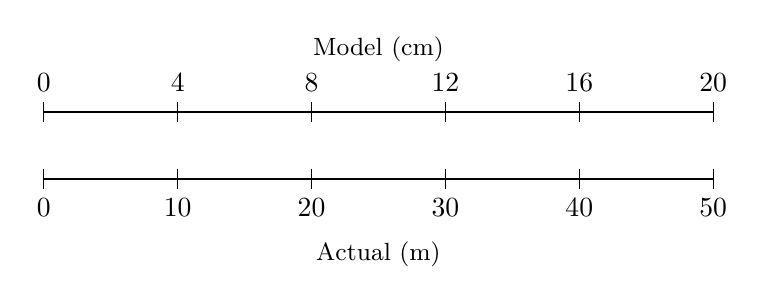
\begin{tikzpicture}[scale=0.85]
  \draw[thick] (0,0.5) -- (10,0.5);
  \draw[thick] (0,-0.5) -- (10,-0.5);
  \foreach \x/\lab in {0/0, 2/4, 4/8, 6/12, 8/16, 10/20}
    \draw (\x,0.35) -- (\x,0.65) node[above]{$\lab$};
  \node[above] at (5,1.1) {\small Model (cm)};
  \foreach \x/\lab in {0/0, 2/10, 4/20, 6/30, 8/40, 10/50}
    \draw (\x,-0.35) -- (\x,-0.65) node[below]{$\lab$};
  \node[below] at (5,-1.3) {\small Actual (m)};
\end{tikzpicture}
\end{center}

What actual length corresponds to a model length of $14$ cm?
\end{questionText}
\choiceA{$28$ m}
\choiceB{$35$ m}
\choiceC{$42$ m}
\choiceD{$70$ m}
\correctAnswer{B}
\explanation{From the double number line, the ratio is $\frac{10}{4} = 2.5$ m per cm. For $14$ cm: $14 \times 2.5 = 35$ m.}
\end{practiceQuestion}

\begin{practiceQuestion}{1-7-q24}{gmc}
\begin{questionText}
The table below shows model and actual dimensions for a scale model ship.

\begin{center}
\begin{tabular}{|c|c|}
\hline
\textbf{Model (cm)} & \textbf{Actual (m)} \\
\hline
$5$ & $10$ \\
$12$ & $24$ \\
$18$ & $36$ \\
$25$ & $?$ \\
\hline
\end{tabular}
\end{center}

What is the actual measurement for a model measurement of $25$ cm?
\end{questionText}
\choiceA{$37$ m}
\choiceB{$45$ m}
\choiceC{$50$ m}
\choiceD{$125$ m}
\correctAnswer{C}
\explanation{Scale factor: $\frac{10}{5} = 2$ m per cm (which means each cm on the model $= 2$ m in real life, or $200$ cm, giving a scale of $1 : 200$). For $25$ cm: $25 \times 2 = 50$ m.}
\end{practiceQuestion}

% --- Graphical Short Answer Questions (3) ---

\begin{practiceQuestion}{1-7-q25}{gsa}
\begin{questionText}
The scale drawing below shows the outline of a rectangular garden with a walkway across the middle.

\begin{center}
\begin{tikzpicture}[scale=0.8]
  \draw[thick,funGreen,fill=funGreen!10] (0,0) rectangle (6,4);
  \draw[thick,funOrange,fill=funOrange!20] (2.5,0) rectangle (3.5,4);
  \draw[<->,thick] (0,-0.5) -- (6,-0.5) node[midway,below]{\small $6$ cm};
  \draw[<->,thick] (-0.5,0) -- (-0.5,4) node[midway,left]{\small $4$ cm};
  \draw[<->,thick] (2.5,4.4) -- (3.5,4.4) node[midway,above]{\small $1$ cm};
  \node at (1.2,2) {\small Garden};
  \node[rotate=90] at (3,2) {\small Walk};
  \node at (0,-1.3) {};
  \node at (3,-1.3) {\small Scale: $1$ cm $= 3$ m};
\end{tikzpicture}
\end{center}

What is the actual area of the walkway in square meters?
\end{questionText}
\correctAnswer{$36$ sq m}
\explanation{Walkway on drawing: $1$ cm wide $\times$ $4$ cm long. Actual: width $= 1 \times 3 = 3$ m, length $= 4 \times 3 = 12$ m. Area $= 3 \times 12 = 36$ square meters.}
\end{practiceQuestion}

\begin{practiceQuestion}{1-7-q26}{gsa}
\begin{questionText}
The graph below shows the proportional relationship between model dimensions (cm) and actual dimensions (m) for a scale model.

\begin{center}
\begin{tikzpicture}[scale=0.5]
  \draw[step=1,gray!20,thin] (0,0) grid (10,10);
  \draw[thick,->] (0,0) -- (10.5,0) node[right]{\small Model (cm)};
  \draw[thick,->] (0,0) -- (0,10.5) node[above]{\small Actual (m)};
  \foreach \x in {2,4,6,8,10} \draw (\x,0.1) -- (\x,-0.1) node[below]{\tiny \x};
  \foreach \y in {2,4,6,8,10} \draw (0.1,\y) -- (-0.1,\y) node[left]{\tiny \y};
  \draw[thick,funBlue] (0,0) -- (10,8);
  \fill[funBlue] (0,0) circle (3pt);
  \fill[funBlue] (5,4) circle (3pt);
  \fill[funBlue] (10,8) circle (3pt);
\end{tikzpicture}
\end{center}

Using the graph, find the actual dimension for a model measurement of $15$ cm.
\end{questionText}
\correctAnswer{$12$ m}
\explanation{From the point $(5, 4)$: $k = \frac{4}{5} = 0.8$ m per cm. For $15$ cm: $0.8 \times 15 = 12$ m.}
\end{practiceQuestion}

\begin{practiceQuestion}{1-7-q27}{gsa}
\begin{questionText}
A model airplane uses the following scale chart.

\begin{center}
\begin{tabular}{|c|c|}
\hline
\textbf{Model (cm)} & \textbf{Actual (m)} \\
\hline
$3$ & $2.1$ \\
$7$ & $4.9$ \\
$11$ & $7.7$ \\
$16$ & $?$ \\
\hline
\end{tabular}
\end{center}

What is the actual measurement corresponding to $16$ cm on the model?
\end{questionText}
\correctAnswer{$11.2$ m}
\explanation{Find the scale: $\frac{2.1}{3} = 0.7$ m per cm. Verify: $0.7 \times 7 = 4.9$ ✓, $0.7 \times 11 = 7.7$ ✓. For $16$ cm: $0.7 \times 16 = 11.2$ m.}
\end{practiceQuestion}
